15. \begin{figure}[ht!]
\center{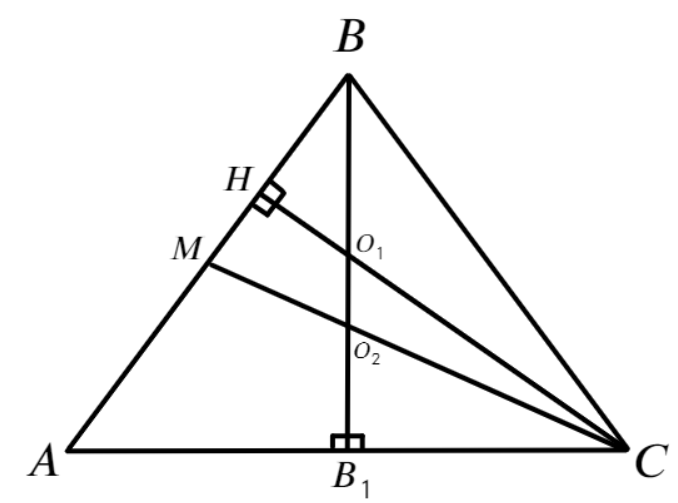
\includegraphics[scale=0.35]{g9-15.png}}
\end{figure}\\
Пусть $CH$ высота, $CM$ медиана, а $BB_1$ --- и то, и другое. По теореме Пифагора $BB_1=\sqrt{5^2-3^2}=4.$ Так как медианы делятся точкой их пересечения в отношении $2:1,$ имеем $O_2B_1=\cfrac{1}{3}\cdot4=\cfrac{4}{3}.$ В четырёхугольнике $B_1HBC$ равны углы $BHC$ и $BB_1C,$ образованные противоположными сторонами и разными диагоналями, значит он является вписанным и поэтому $\angle B_1CO_1=\angle B_1BH.$ Тогда треугольники $CO_1B_1$ и $B_1BA$ подобны по двум углам и  $\cfrac{CB_1}{BB_1}=\cfrac{B_1O_1}{AB_1},\ \cfrac{3}{4}=\cfrac{B_1O_1}{3}\Rightarrow B_1O_1=\cfrac{9}{4}.$ Таким образом, $O_1O_2=B_1O_1-O_2B_1=\cfrac{9}{4}-\cfrac{4}{3}=\cfrac{11}{12}.$\\
